\documentclass{article}
\usepackage{tikz}

\begin{document}

\begin{center}
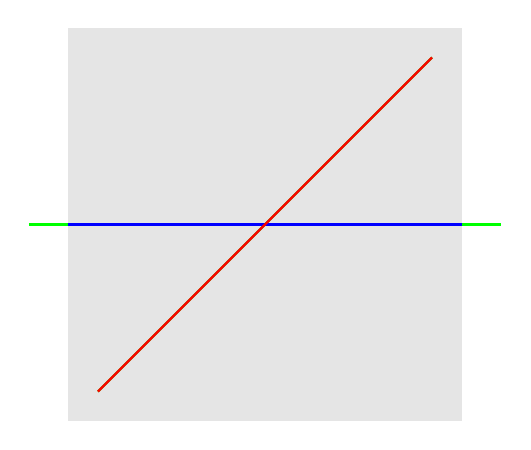
\begin{tikzpicture}
    % Draw a visible clipping area in light gray
    \fill[gray!20] (-2.5,-2.5) rectangle (2.5,2.5);

    % No clipping: Full untrimmed line (green)
    \draw[thick, green] (-3,0) -- (3,0);
    \draw[thick, green, rotate=45] (-3,0) -- (3,0);

    % Apply clipping
    \begin{scope}
        \clip (-2.5,-2.5) rectangle (2.5,2.5);

        % Trimmed version of the lines (blue and red)
        \draw[thick, blue] (-3,0) -- (3,0);
        \draw[thick, red, rotate=45] (-3,0) -- (3,0);
    \end{scope}
\end{tikzpicture}
\end{center}

\end{document}
